%File: formatting-instruction.tex
\documentclass[letterpaper]{article}
\usepackage{aaai}
\usepackage{times}
\usepackage{helvet}
\usepackage{courier}
\usepackage{graphicx}
\usepackage{xcolor}
\usepackage{natbib}
\bibliographystyle{aaai}
% Sudo Code packages
\usepackage[ruled, linesnumbered]{algorithm2e}

\usepackage{amsfonts}

\graphicspath{../../}

\frenchspacing
\setlength{\pdfpagewidth}{8.5in}
\setlength{\pdfpageheight}{11in}
\pdfinfo{
/Title (Reinforcement Learning: Parking lot)
/Author (Robert Horton)}
\setcounter{secnumdepth}{0}  
 \begin{document}

% The file aaai.sty is the style file for AAAI Press 
% proceedings, working notes, and technical reports.
%
\title{Reinforcement Learning\\ Artificial Neural Network: Valet Parking Lot }
\author{Robert Horton\\
UCCS\\
1420 Austin Bluffs Pkwy,\\
Colorado Springs, Colorado 80918\\
}
\maketitle

% ----------------------------------------------- Abstract
\begin{abstract}
\begin{quote}
In society when considering segregation amongst several different groups there seems to be just as many physiological phenomenons as there are seemingly counter intuitive revelations.Through coded implementation, an instance of a randomly generated  graph can be generated to run \textit{contentedness}.  With varying parameter values, we analyse dynamic graph interactions amongst agents in a society with spatial awareness of neighbours within a set distance of direct neighbours.   
\end{quote}
\end{abstract}

% ----------------------------------------------- Introduction
\section{Introduction}

\begin{center}
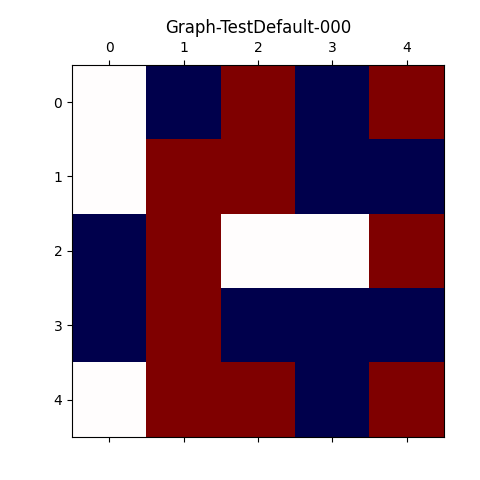
\includegraphics[scale=0.7]{./Content/GenoratedGraphs/Graph-TestDefault-0.1-0.5-0.2/Graph-TestDefault-000}
\end{center}

% ----------------------------------------------- Implementation
\section{Implementation}  

Book for the class  (\cite{10.5555/1805895})\\
web site for python (\cite{AdilMoujahid})\\
paper for segregation with graphs (\cite{ijcai2019-38})\\

% ----------------------- Execution 
\subsection{Execution}

% ----------------------- Analyisis 
\subsection{Analyisis}
 
% ----------------------------------------------- Conclusion
\section{Conclusion}

% ----------------------------------------------- References 

\bibliography{ArticleTemplate}

\end{document}